%\section{Anhang}\label{anhang}
\subsection{Konfigurationsdateien}

	\lstinputlisting[caption={package.json für das GFB-Testprojekt}, label=lst:gfb-package]{lst/gfb/package.json}

	\newpage
	\lstinputlisting[caption={karma.conf.js für das GFB-Testprojekt}, label=lst:gfb-karma]{lst/gfb/karma.conf.js}

	\newpage
	\lstinputlisting[caption={protractor.conf.js für das GFB-Testprojekt}, label=lst:gfb-protractorConf]{lst/gfb/protractor.conf.js}

\newpage
\subsection{Testsuites}
	\lstinputlisting[caption={test/spec/test\_spec.js}, label=lst:gfb-valid1]{test/spec/test_spec.js}
	
	\newpage
	\lstinputlisting[caption={test/spec/ngTest\_spec.js}, label=lst:gfb-valid2]{test/spec/ngTest_spec.js}

	\newpage
	\lstinputlisting[caption={test/spec/overviewCtrl\_spec.js}, label=lst:gfb-overviewCtrl]{test/spec/overviewCtrl_spec.js}

	\newpage
	\lstinputlisting[caption={test/spec/svc\_obs\_spec.js}, label=lst:gfb-svc_obs]{test/spec/svc_obs_spec.js}

	\newpage
	\lstinputlisting[caption={test/spec/dir\_filHb\_spec.js}, label=lst:gfb-dir_filHb]{test/spec/dir_filHb_spec.js}

	\newpage
	\lstinputlisting[caption={test/spec/uniqueFilter\_spec.js}, label=lst:gfb-unique]{test/spec/uniqueFilter_spec.js}

	\newpage
	\lstinputlisting[caption={test/e2e/test\_spec.js}, label=lst:gfb-protractorTest]{lst/gfb/test/e2e/test_spec.js}

\newpage
\subsection{Sonstiges}
\begin{figure}[H]
	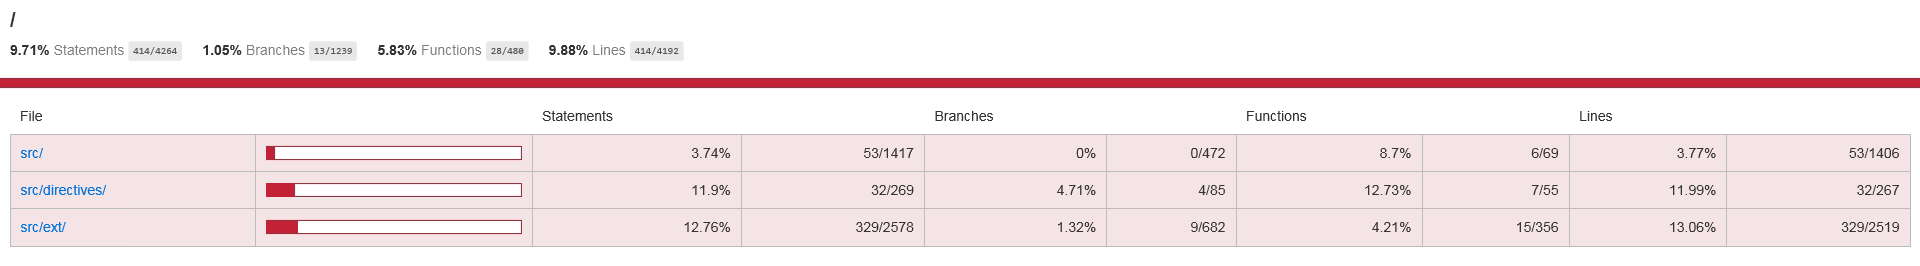
\includegraphics[width=\textwidth]{abb/code-cov-1.png}
	\caption{Übersichtsseite des Code-Coverage-Berichts im Browser}
	\label{abb:code-cov-1}
\end{figure}

\begin{figure}[H]
	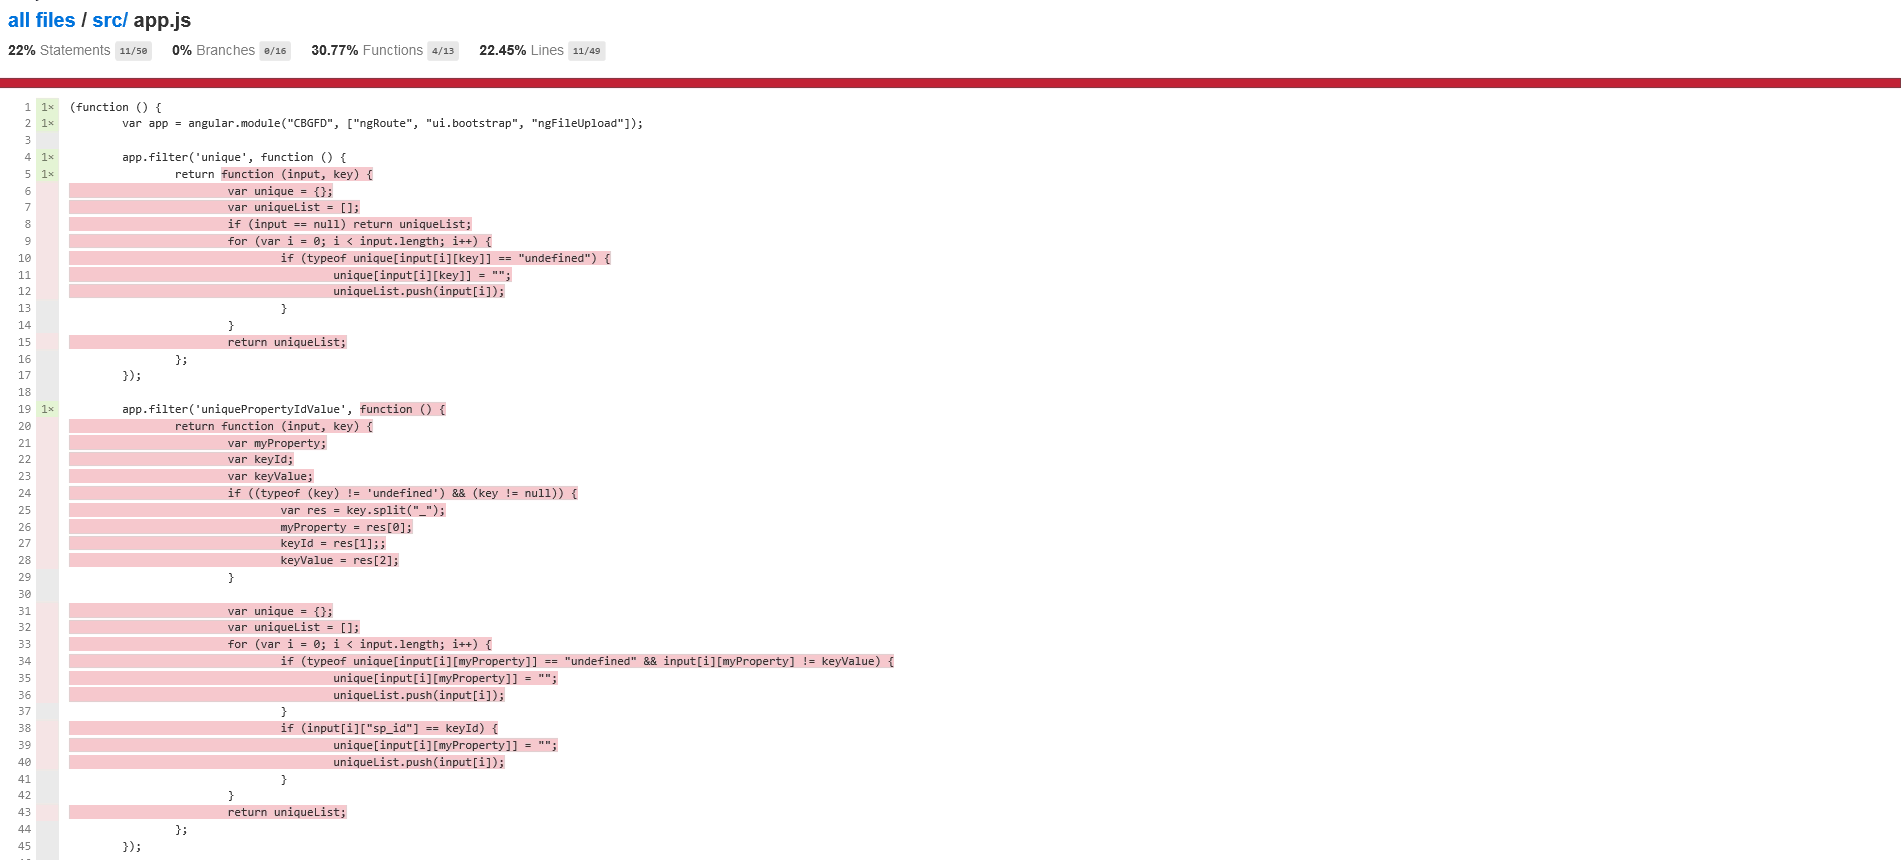
\includegraphics[width=\textwidth]{abb/code-cov-2.png}
	\caption[Detailseite des Code-Coverage-Berichts im Browser]{Detailseite des Code-Coverage-Berichts im Browser (Der abgebildete Quelltext ist Teil des GFB-Projekts und damit Eigentum der \domain)}
	\label{abb:code-cov-2}
\end{figure}

\begin{figure}[H]
	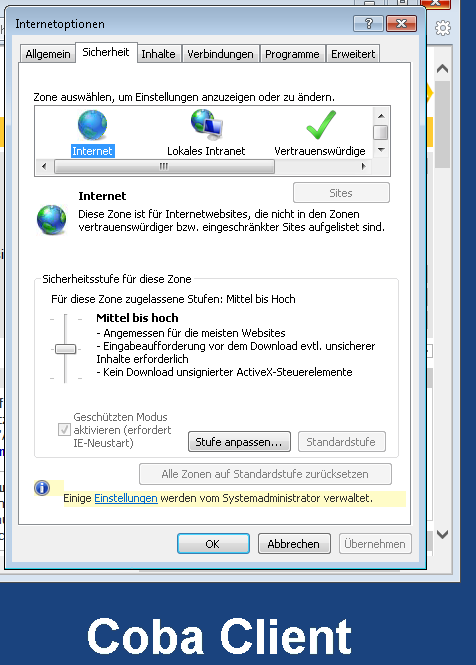
\includegraphics[width=0.8\textwidth]{abb/coba-ie.png}
	\caption{Einstellungsdialog zur Deakitiverung des Geschützten Modus' an einem Commerzbank-Arbeitsplatz}
	\label{abb:coba-ie}
\end{figure}